\documentclass[a4paper, 11pt]{article}
\author{Kajetan Kaczmarek}
\usepackage{amsmath}
\usepackage{graphicx}
\usepackage{listings}
\usepackage[T1]{fontenc}
\usepackage[utf8]{inputenc}
\usepackage[polish]{babel}
\usepackage{color} %red, green, blue, yellow, cyan, magenta, black, white
\definecolor{mygreen}{RGB}{28,172,0} % color values Red, Green, Blue
\definecolor{mylilas}{RGB}{170,55,241}


\lstset{language=Matlab,%
    %basicstyle=\color{red},
    breaklines=true,%
    morekeywords={matlab2tikz},
    keywordstyle=\color{blue},%
    morekeywords=[2]{1}, keywordstyle=[2]{\color{black}},
    identifierstyle=\color{black},%
    stringstyle=\color{mylilas},
    commentstyle=\color{mygreen},%
    showstringspaces=false,%without this there will be a symbol in the places where there is a space
    numbers=left,%
    numberstyle={\tiny \color{black}},% size of the numbers
    numbersep=9pt, % this defines how far the numbers are from the text
    emph=[1]{for,end,break},emphstyle=[1]\color{red}, %some words to emphasise
    %emph=[2]{word1,word2}, emphstyle=[2]{style},    
}



\begin{document}
\title{Sprawozdanie MNUM \\* Projekt nr.2 \\* 
Zadanie 2.24 \\*}
\maketitle

\begin{enumerate}

\item Opis zastosowanych algorytmów : 
\begin{enumerate}
\item W pierwszym zadaniu zaimplementowałem algorytm przeprowadzający faktoryzację QR danej macierzy. Program przyjmuje jako wartości wejściowe tolerancję, macierz do faktoryzacji oraz maksymalną ilość iteracji po których działanie programu ma być przerwane.Metoda bez przesunięć iterowała faktoryzacjęQR i następnie korzystała ze wzoru 
\[ A = R*Q\]
\item Przy drugim poleceniu zrealizowałem algorytm aproksymacji funkcji przez metodę namniejszych kwadratów.Dla próbek
\begin{center}
\begin{tabular}{ l*{2}{c}r}
  \hline			
\bfseries Y & X \\
\bfseries -5.4606 & -5 \\
\bfseries -3.8804 & -4 \\
\bfseries -1.9699 & -3 \\
\bfseries -1.6666 & -2 \\
\bfseries -0.0764 & -1 \\
\bfseries -0.3971 & 0 \\
\bfseries -1.0303 & 1 \\
\bfseries -4.5483 & 2 \\
\bfseries -11.5280  & 3 \\
\bfseries -21.6417 & 4 \\
\bfseries -34.4458 & 5 \\
  \hline  
\end{tabular}
\end{center}
\bigskip

zastosowałem dwa warianty algorytmu:
\begin{itemize}
\item Z użyciem układu równań normalnych, tj. \[ A^{T}Ax = A^{T}b\]
\item Z użyciem układu równań liniowych z macierzą R powstałą na skutek rozkładu QR, tj.
\[ Rx = Q^{T}b\]
\end{itemize}
\item Kod moich programów 
\begin{itemize}
\item Kod główny pierwszego programu
\lstinputlisting{P1_Main.m}
\item Faktoryzacja QR
\lstinputlisting{Factorize_QR.m}
\item Użycie faktoryzacji QR do znalezienia wartości własnych macierzy bez przesunięć
\lstinputlisting{QR_Factorization_NoShift.m}
\item Użycie faktoryzacji QR do znalezienia wartości własnych macierzy z przesunięciami
\lstinputlisting{QR_Factorization_Shift.m}
\item Kod główny drugiego programu
\item Użycie faktoryzacji QR do znalezienia wartości własnych macierzy bez przesunięć
\lstinputlisting{P2_Main.m}
\item LLSP z użyciem równań normalnych
\lstinputlisting{LLSPNormals.m}
\item LLSP z użyciem faktoryzacji QR
\lstinputlisting{LLSPQR.m}
\end{itemize}
\item
Wyniki : 
\begin{itemize}
\item Wyniki QR
\begin{center}
\begin{tabular}{ l*{2}{c}r}
\hline
\bfseries Rozmiar macierzy & Metoda & Średnia ilość iteracji \\
\bfseries 5 & Bez przesunięć & 72.5\\
\bfseries 5 & Z przesunięciami & 7.33\\
\bfseries 5 & Z przesunięciami Asymetryczna & 9.53\\
\bfseries 10 & Bez przesunięć & 215.46\\
\bfseries 10 & Z przesunięciami & 14.10\\
\bfseries 10 & Z przesunięciami Asymetryczna & 21\\
\bfseries 20 & Bez przesunięć & 1824.4\\
\bfseries 20 & Z przesunięciami & 28.87\\
\bfseries 20 & Z przesunięciami Asymetryczna & 44.73\\
\hline  
\end{tabular}
\end{center}
\bigskip

\item Wyniki LLSP
\begin{center}
\begin{tabular}{ l*{2}{c}r}
  \hline	
  \bfseries N & Norma Euklidesowa & Norma Czebyszewa\\
  \bfseries 1 & 34.3326 & 26.5690 \\
  \bfseries 2 & 24.5832 & 15.1424 \\
  \bfseries 3 & 7.3647 & 3.1643 \\
    \bfseries 4 & 1.4390 & 0.6769 \\
      \bfseries 5 & 1.3958 & 0.6486 \\
        \bfseries 6 & 0.8501 & 0.4642 \\
        \bfseries 7 & 0.7595 & 0.4239 \\
  \bfseries 8 & 0.7069 & 0.4448 \\
  \bfseries 9 & 0.7410 & 0.4819 \\

  \hline  
\end{tabular}
\end{center}
\bigskip

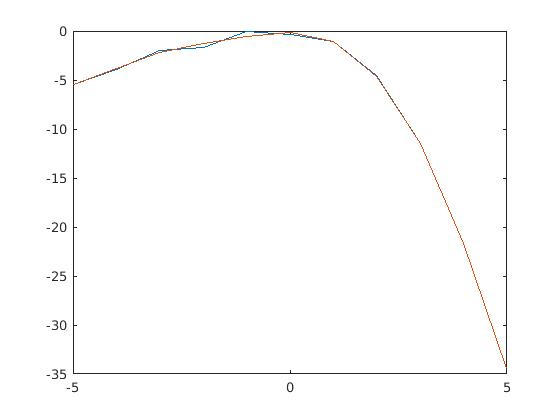
\includegraphics[width=\textwidth, height=\textheight, keepaspectratio]{/home/kajkacz/Documents/MNUM/ProjektNr.2/Aprr.jpg}

\end{itemize}
\item Wnioski : Obydwie metody wydają się oferować dostateczną precyzję. Dla odpowiednio dużej ilości iteracji lub odpowiednio wysokim stopniu wielomianu metody sprawdzają się.Widać także że wraz ze wzrostem macierzy metoda wyznaczania wartości własnych bez przesunięcia staje się zdecydowanie wolniejsza

\end{enumerate}
\end{enumerate}
\end{document}

